\subsection{Systèmes modulaires}

\begin{frame}[c]{Exemples de systèmes modulaires}
    \vfill
    \begin{columns}[c,totalwidth=\textwidth]
        \column{0.6\textwidth}
        \textbf{Systèmes non autonomes :}
        \begin{itemize}
            \item \textbf{DRAGON Drone} \cite{zhao_design_2018} : modules articulés, modification de forme
        \end{itemize}
        
        \textbf{Systèmes autonomes :}
        \begin{itemize}
            \item \textbf{ModQuad} \cite{saldana_modquad_2018} : quadricoptères avec accrochage magnétique
            \item \textbf{TRADY} \cite{sugihara_design_2023} : aimants commutables + ergots
            \item \textbf{BEATLE} \cite{sugihara_beatle_2024} : contrôle distribué
            \item \textbf{LEGION} \cite{junichiro_workshop_2025} : système tri-coptères
        \end{itemize}
        
        \column{0.35\textwidth}
        \begin{figure}
            \centering
            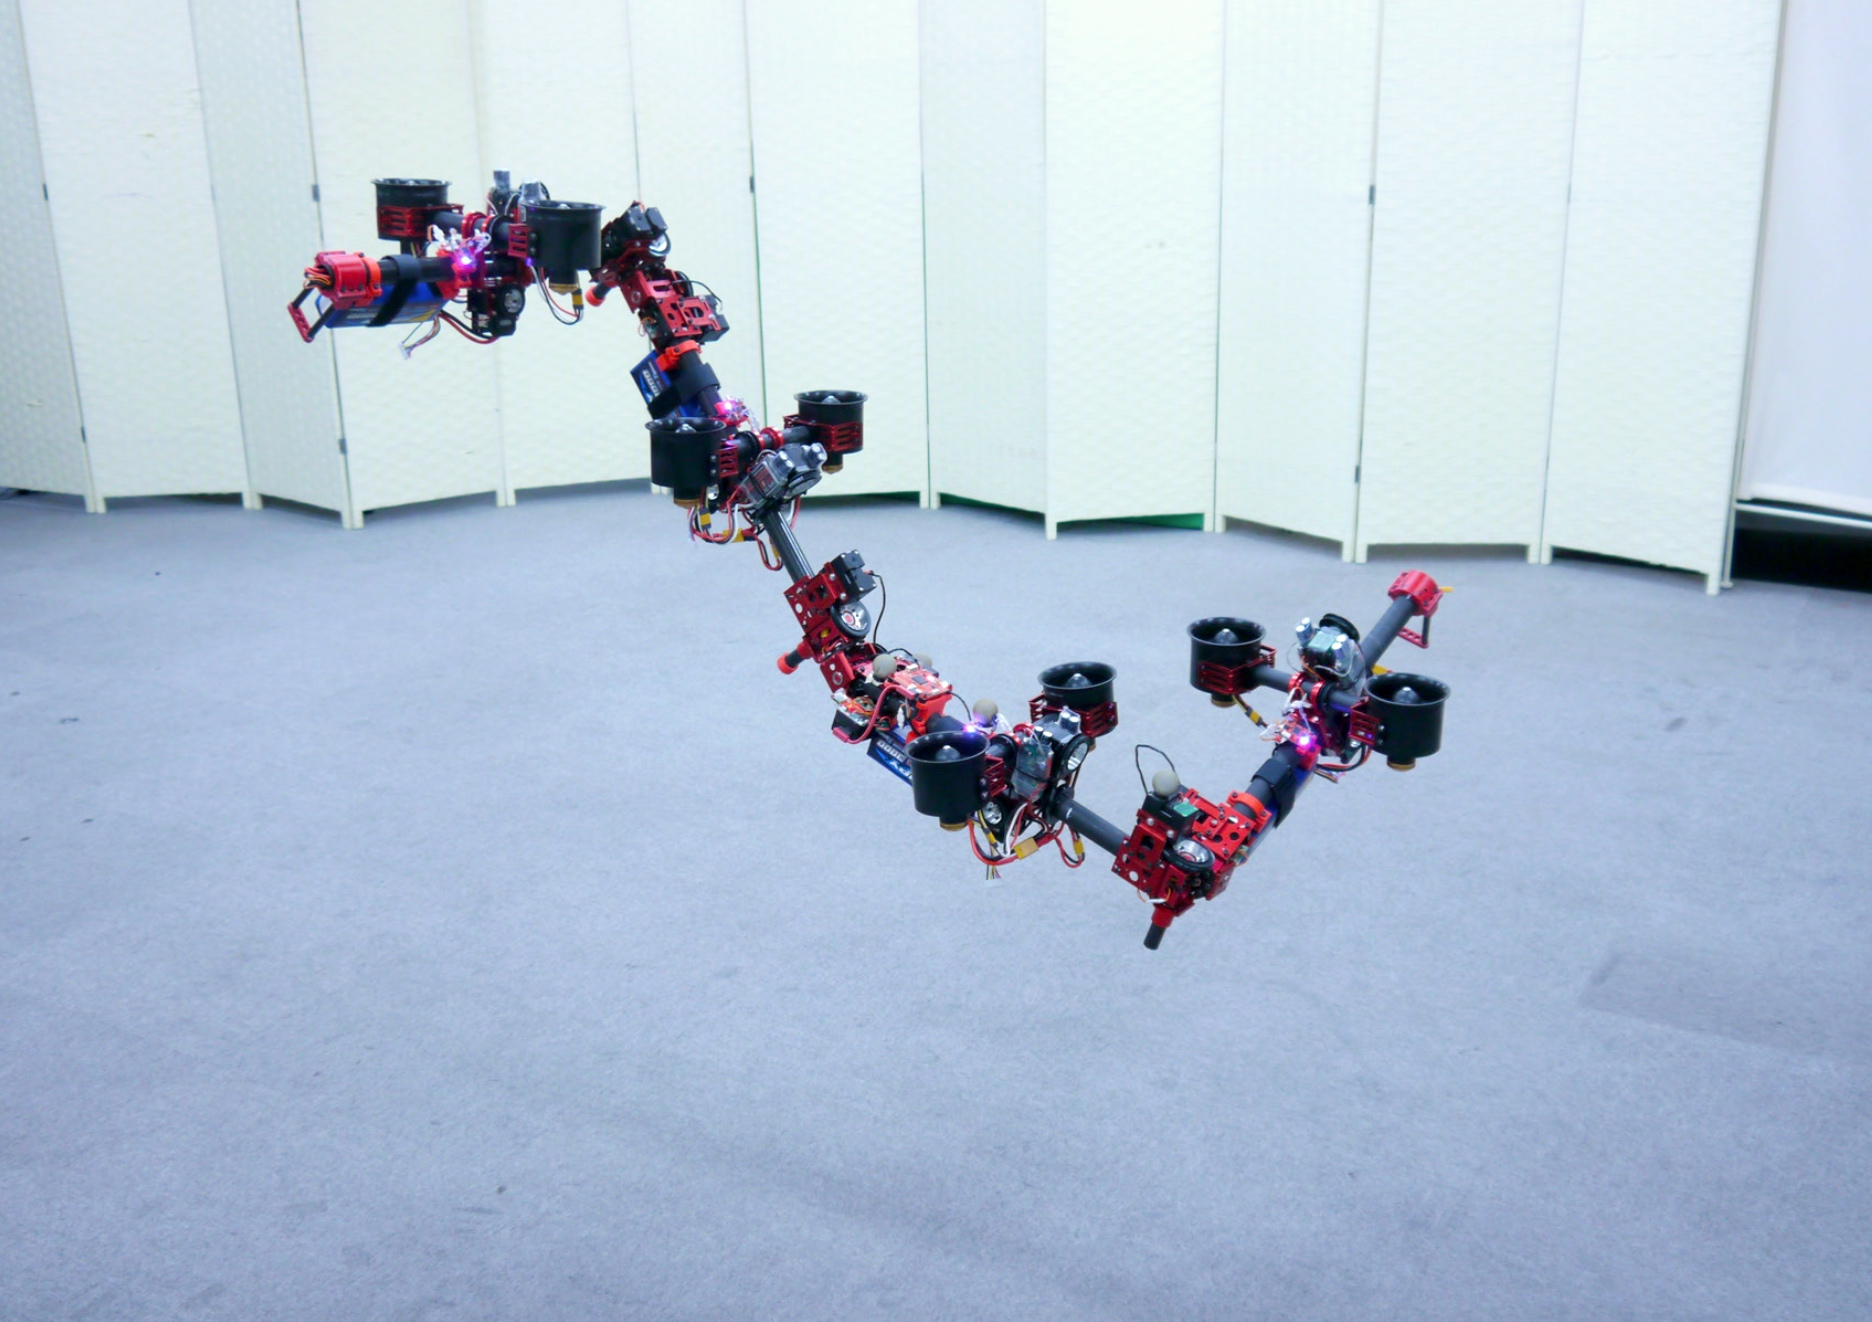
\includegraphics[width=0.8\linewidth]{3-etat-de-lart/pic/dragon-drone.jpeg}
            \caption{DRAGON Drone}
        \end{figure}
        \vspace{0.3cm}
        \begin{figure}
            \centering
            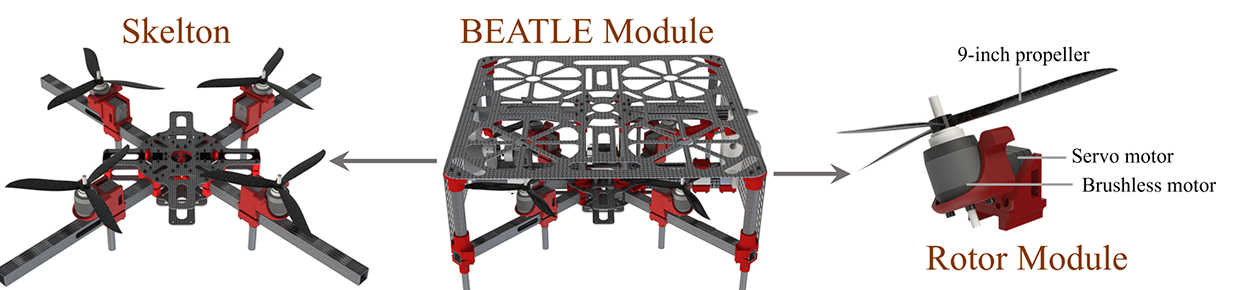
\includegraphics[width=0.8\linewidth]{3-etat-de-lart/pic/beatle.png}
            \caption{BEATLE}
        \end{figure}
    \end{columns}
    \vfill
\end{frame}

